% Options for packages loaded elsewhere
\PassOptionsToPackage{unicode}{hyperref}
\PassOptionsToPackage{hyphens}{url}
%
\documentclass[
]{book}
\usepackage{lmodern}
\usepackage{amssymb,amsmath}
\usepackage{ifxetex,ifluatex}
\ifnum 0\ifxetex 1\fi\ifluatex 1\fi=0 % if pdftex
  \usepackage[T1]{fontenc}
  \usepackage[utf8]{inputenc}
  \usepackage{textcomp} % provide euro and other symbols
\else % if luatex or xetex
  \usepackage{unicode-math}
  \defaultfontfeatures{Scale=MatchLowercase}
  \defaultfontfeatures[\rmfamily]{Ligatures=TeX,Scale=1}
\fi
% Use upquote if available, for straight quotes in verbatim environments
\IfFileExists{upquote.sty}{\usepackage{upquote}}{}
\IfFileExists{microtype.sty}{% use microtype if available
  \usepackage[]{microtype}
  \UseMicrotypeSet[protrusion]{basicmath} % disable protrusion for tt fonts
}{}
\makeatletter
\@ifundefined{KOMAClassName}{% if non-KOMA class
  \IfFileExists{parskip.sty}{%
    \usepackage{parskip}
  }{% else
    \setlength{\parindent}{0pt}
    \setlength{\parskip}{6pt plus 2pt minus 1pt}}
}{% if KOMA class
  \KOMAoptions{parskip=half}}
\makeatother
\usepackage{xcolor}
\IfFileExists{xurl.sty}{\usepackage{xurl}}{} % add URL line breaks if available
\IfFileExists{bookmark.sty}{\usepackage{bookmark}}{\usepackage{hyperref}}
\hypersetup{
  pdftitle={Reproducible Medical Research with R},
  pdfauthor={Peter D.R. Higgins, MD, PhD, MSc},
  hidelinks,
  pdfcreator={LaTeX via pandoc}}
\urlstyle{same} % disable monospaced font for URLs
\usepackage{color}
\usepackage{fancyvrb}
\newcommand{\VerbBar}{|}
\newcommand{\VERB}{\Verb[commandchars=\\\{\}]}
\DefineVerbatimEnvironment{Highlighting}{Verbatim}{commandchars=\\\{\}}
% Add ',fontsize=\small' for more characters per line
\usepackage{framed}
\definecolor{shadecolor}{RGB}{248,248,248}
\newenvironment{Shaded}{\begin{snugshade}}{\end{snugshade}}
\newcommand{\AlertTok}[1]{\textcolor[rgb]{0.94,0.16,0.16}{#1}}
\newcommand{\AnnotationTok}[1]{\textcolor[rgb]{0.56,0.35,0.01}{\textbf{\textit{#1}}}}
\newcommand{\AttributeTok}[1]{\textcolor[rgb]{0.77,0.63,0.00}{#1}}
\newcommand{\BaseNTok}[1]{\textcolor[rgb]{0.00,0.00,0.81}{#1}}
\newcommand{\BuiltInTok}[1]{#1}
\newcommand{\CharTok}[1]{\textcolor[rgb]{0.31,0.60,0.02}{#1}}
\newcommand{\CommentTok}[1]{\textcolor[rgb]{0.56,0.35,0.01}{\textit{#1}}}
\newcommand{\CommentVarTok}[1]{\textcolor[rgb]{0.56,0.35,0.01}{\textbf{\textit{#1}}}}
\newcommand{\ConstantTok}[1]{\textcolor[rgb]{0.00,0.00,0.00}{#1}}
\newcommand{\ControlFlowTok}[1]{\textcolor[rgb]{0.13,0.29,0.53}{\textbf{#1}}}
\newcommand{\DataTypeTok}[1]{\textcolor[rgb]{0.13,0.29,0.53}{#1}}
\newcommand{\DecValTok}[1]{\textcolor[rgb]{0.00,0.00,0.81}{#1}}
\newcommand{\DocumentationTok}[1]{\textcolor[rgb]{0.56,0.35,0.01}{\textbf{\textit{#1}}}}
\newcommand{\ErrorTok}[1]{\textcolor[rgb]{0.64,0.00,0.00}{\textbf{#1}}}
\newcommand{\ExtensionTok}[1]{#1}
\newcommand{\FloatTok}[1]{\textcolor[rgb]{0.00,0.00,0.81}{#1}}
\newcommand{\FunctionTok}[1]{\textcolor[rgb]{0.00,0.00,0.00}{#1}}
\newcommand{\ImportTok}[1]{#1}
\newcommand{\InformationTok}[1]{\textcolor[rgb]{0.56,0.35,0.01}{\textbf{\textit{#1}}}}
\newcommand{\KeywordTok}[1]{\textcolor[rgb]{0.13,0.29,0.53}{\textbf{#1}}}
\newcommand{\NormalTok}[1]{#1}
\newcommand{\OperatorTok}[1]{\textcolor[rgb]{0.81,0.36,0.00}{\textbf{#1}}}
\newcommand{\OtherTok}[1]{\textcolor[rgb]{0.56,0.35,0.01}{#1}}
\newcommand{\PreprocessorTok}[1]{\textcolor[rgb]{0.56,0.35,0.01}{\textit{#1}}}
\newcommand{\RegionMarkerTok}[1]{#1}
\newcommand{\SpecialCharTok}[1]{\textcolor[rgb]{0.00,0.00,0.00}{#1}}
\newcommand{\SpecialStringTok}[1]{\textcolor[rgb]{0.31,0.60,0.02}{#1}}
\newcommand{\StringTok}[1]{\textcolor[rgb]{0.31,0.60,0.02}{#1}}
\newcommand{\VariableTok}[1]{\textcolor[rgb]{0.00,0.00,0.00}{#1}}
\newcommand{\VerbatimStringTok}[1]{\textcolor[rgb]{0.31,0.60,0.02}{#1}}
\newcommand{\WarningTok}[1]{\textcolor[rgb]{0.56,0.35,0.01}{\textbf{\textit{#1}}}}
\usepackage{longtable,booktabs}
% Correct order of tables after \paragraph or \subparagraph
\usepackage{etoolbox}
\makeatletter
\patchcmd\longtable{\par}{\if@noskipsec\mbox{}\fi\par}{}{}
\makeatother
% Allow footnotes in longtable head/foot
\IfFileExists{footnotehyper.sty}{\usepackage{footnotehyper}}{\usepackage{footnote}}
\makesavenoteenv{longtable}
\usepackage{graphicx,grffile}
\makeatletter
\def\maxwidth{\ifdim\Gin@nat@width>\linewidth\linewidth\else\Gin@nat@width\fi}
\def\maxheight{\ifdim\Gin@nat@height>\textheight\textheight\else\Gin@nat@height\fi}
\makeatother
% Scale images if necessary, so that they will not overflow the page
% margins by default, and it is still possible to overwrite the defaults
% using explicit options in \includegraphics[width, height, ...]{}
\setkeys{Gin}{width=\maxwidth,height=\maxheight,keepaspectratio}
% Set default figure placement to htbp
\makeatletter
\def\fps@figure{htbp}
\makeatother
\setlength{\emergencystretch}{3em} % prevent overfull lines
\providecommand{\tightlist}{%
  \setlength{\itemsep}{0pt}\setlength{\parskip}{0pt}}
\setcounter{secnumdepth}{5}
\usepackage{booktabs}
\usepackage{amsthm}
\makeatletter
\def\thm@space@setup{%
  \thm@preskip=8pt plus 2pt minus 4pt
  \thm@postskip=\thm@preskip
}
\makeatother
\usepackage[]{natbib}
\bibliographystyle{apalike}

\title{Reproducible Medical Research with R}
\author{Peter D.R. Higgins, MD, PhD, MSc}
\date{2020-05-26}

\begin{document}
\maketitle

{
\setcounter{tocdepth}{1}
\tableofcontents
}
\hypertarget{preface}{%
\chapter{Preface}\label{preface}}

Welcome to Reproducible Medical Research with R (RMWR). I hope that this book meets your needs.

\hypertarget{who-this-book-is-for}{%
\section{Who This Book is For}\label{who-this-book-is-for}}

This is a book for anyone in the medical field interested in analyzing the data available to them to better understand health, disease, or delivery of care. This could include nurses, dieticians, psychologists, and PhDs in related fields, as well as medical students, residents, fellows, or doctors in practice.\\
I expect that most learners will be using this book in their spare time at night and on weekends, as the medical school curriculum is already packed full, and there is no room to add skills in reproducible research to the standard curriculum. This book is designed for self-teaching, and many hints and solutions will be provided to avoid roadblocks and frustration.
Many learners find themselves wanting to develop reproducible research skills after they have finished their training, and after they have become comfortable with their clinical role. This is the time when they identify and want to address problems in their practice with the data they have before them. This book is for you.

\hypertarget{prerequisites}{%
\section{Prerequisites}\label{prerequisites}}

Thank you for giving this e-book a try. This is designed for physicians or others analyzing health data who are interested in pursuing this field using the R language.
We will assume that:

\begin{itemize}
\tightlist
\item
  you have access to a computer
\item
  that you have access to the internet
\item
  that you can download the current version of R, and
\item
  that you have downloaded a current version of Rstudio.
\end{itemize}

\hypertarget{the-spiral-of-success-structure}{%
\section{The Spiral of Success Structure}\label{the-spiral-of-success-structure}}

This book is structured on the concept of a ``spiral of success'', with readers learning about topics like data visualization, data wrangling, data modeling, reproducible research, and communication of results in repeated passes. These will initially be at a superficial level, and at each pass of the spiral, will provide increasing depth and complexity. This means that the chapters on data wrangling will not all be together, nor the chapters on data visualization. Our goal is to build skills gradually, and return to (and remind students of) their previously built skills in one area and to add to them. The eventual goal is for learners to be able to produce, document, and communicate reproducible research to their community.

\hypertarget{motivation-for-this-book}{%
\section{Motivation for this Book}\label{motivation-for-this-book}}

Most medical people who learn R to do their own data analysis do it on their own time. They rarely have time for a semester-long course, and their clinical schedules usually will not allow it. Fortunately, a lot of people learn R on their own, and there is a strong and supportive R Community to help new learners. A 2019 Twitter survey conducted by \texttt{@RLadies} found that more than half of respondents were largely self-taught, from books and online resources.

There are a lot of good resources for learning R, so why one more? In part, because the needs of a medical audience are often different. There are distinct needs for protecting health information, generating a descriptive Table One, using secure data tools like REDCap, and creating standard medical journal and meeting output in Word, Powerpoint, and poster formats.

More and more, all science is becoming data science. We are able to track patients, their test results, and even the individual pixels (voxels) of their CT scans electronically, and use those data points to develop new knowledge. While one could argue that health care workers should collect data and bring it to trained statisticians, this does not work nearly as well as you might expect. Most academic statisticians are incentivized to develop new statistical methods, and are not very interested (or incentivized) to do the hand-holding required to wrangle messy clinical data into a manuscript.

There also are simply not enough statisticians to meet the needs of medical science. Having clinicians on the front lines with some data science training makes a big difference, whether in 1854 in London (John Snow) or in 2014 in Flint, Michigan (Mona Hanna-Atisha). Having more clinicians with some training will impact medical care, as they will identify local problems that would have otherwise never reached a statistician, and probably never been addressed with data otherwise.

\hypertarget{the-scientific-reproducibility-crisis}{%
\section{The Scientific Reproducibility Crisis}\label{the-scientific-reproducibility-crisis}}

Beginning as far back as 1989, with the David Baltimore case, and increasingly publicly through the 2010s, there has been a rising tide of realization that a lot of taxpayer-funded science is done sloppily, and that our standards as scientists need to be higher. The line between carelessly-done science and outright fraud is a thin one, and the case can be made that doing science in a sloppy fashion defrauds the funders, as it leads to results that can not be reproduced nor replicated. Particularly in medicine, where incorrect findings can cause great harm, we should take special care to do scientific research which is well-documented, reproducible, and replicable. This topic as a motivating force for doing careful medical research will be expanded upon in Chapter 1.

\hypertarget{what-this-book-is-not}{%
\section{What this Book is Not}\label{what-this-book-is-not}}

\hypertarget{this-book-is-not-a-statistics-text}{%
\subsection{This Book is Not A Statistics Text}\label{this-book-is-not-a-statistics-text}}

This is not an introduction to statistics. I am assuming that you have learned some statistics somewhere in secondary school, undergraduate studies, graduate school, or even medical school. There are lots of statisticians with Ph.D.s who can certainly teach statistics much more effectively than I can. While I have a master's degree in Clinical Research Design and Statistical Analysis (isn't that a mouthful!) from the University of Michigan, I will leave formal teaching of statistics to the pros.

If you need to brush up on your statistics, no worries. There are several excellent (and free!) e-books on that very topic, using R. Some good examples include (go ahead and click through the blue links to explore):

\begin{enumerate}
\def\labelenumi{\arabic{enumi}.}
\tightlist
\item
  \href{https://learningstatisticswithr-bookdown.netlify.com}{Learning Statistics with R (LSR)}
\item
  \href{https://bookdown.org/fjmcgrade/ismaykim/}{Modern Dive}
\item
  \href{https://tinystats.github.io/teacups-giraffes-and-statistics/index.html}{Teacup Giraffes}
\end{enumerate}

We will cover a lot of the same materials as these books, but with a less theoretical and more applied approach. I will focus on specific medical examples, and emphasize issues (like Protected Health Information) that are particularly important for medical data. I am assuming that you are here because you want to analyze your own data in your probably very limited free time.

\hypertarget{this-book-does-not-provide-comprehensive-coverage-of-the-r-universe}{%
\subsection{This Book Does Not Provide Comprehensive Coverage of the R Universe}\label{this-book-does-not-provide-comprehensive-coverage-of-the-r-universe}}

This book is also far from comprehensive in teaching what is available in the R ecosystem. This book should be considered a launch pad. Many of the later chapters will give you a taste of what is available in certain areas, and guide you to resources (and links) that you can explore to learn more and do more beyond the scope of this book.

\hypertarget{some-guideposts}{%
\section{Some Guideposts}\label{some-guideposts}}

Keep an eye out for Guideposts, which look like this:

\textbf{Warnings}

This is a common gotcha. Watch out for this.

\textbf{Tips}

This is a helpful tip for debugging.

\textbf{Try It Out}

Take what you have learned and try it yourself in the code box below.

\textbf{Challenge} - take the next step and try a more challenging example.

Try this more complicated example.

\textbf{Explore More} - resources for learning more about a particular topic.

If you want to learn more about Shiny apps, go to \url{https://mastering-shiny.org} to see an entire book on the topic.

\hypertarget{getting-started-and-installing-your-tools}{%
\chapter{Getting Started and Installing Your Tools}\label{getting-started-and-installing-your-tools}}

One of the most intimidating parts of getting started with something new is the actual getting started part. Don't worry, we will walk you through this step-by step.

\hypertarget{goals-for-this-chapter}{%
\section{Goals for this Chapter}\label{goals-for-this-chapter}}

\begin{itemize}
\tightlist
\item
  Install R on your Computer
\item
  Install RStudio on your Computer
\item
  Install Git on your Computer
\item
  Get Acquainted with the RStudio IDE
\end{itemize}

\hypertarget{website-links-needed-for-this-chapter}{%
\section{Website links needed for this Chapter}\label{website-links-needed-for-this-chapter}}

While in many chapters, we will list the R packages you need, in this chapter, you will be downloading and installing new software, so we will list the links here for your reference

\begin{itemize}
\tightlist
\item
  \url{https://www.r-project.org}
\item
  \url{https://rstudio.com/products/rstudio/download/}
\item
  \url{https://git-scm.com/downloads}
\end{itemize}

\hypertarget{pathway-for-this-chapter}{%
\section{Pathway for this Chapter}\label{pathway-for-this-chapter}}

This Chapter is part of the \textbf{TOOLS} pathway.
Chapters in this pathway include

\begin{itemize}
\tightlist
\item
  Getting Started and Installing Your Tools
\item
  Updating R, RStudio, and Your Packages
\item
  Advanced Use of the RStudio IDE
\item
  When You Don't Want to Update Packages (Using \emph{renv})
\item
  Major R Updates (Where Are My Packages?)
\end{itemize}

\hypertarget{installing-r-on-your-computer}{%
\section{Installing R on your Computer}\label{installing-r-on-your-computer}}

R is a statistical programming language, designed for non-programmers (statisticians). It is optimized to work with data in tables. It is a very fast and powerful programming engine, but it is not terribly comfortable or convenient. R itself is not terribly user-friendly. It is a lot like a drag racing car, which is basically a person with a steering wheel strapped to an airplane engine.
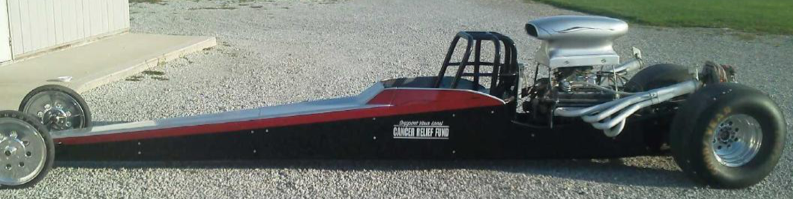
\includegraphics{images/drag.png}
Very aerodynamic and fast, but not comfortable for the long run (more than about 8 seconds).
You will need something more like a production car, with a nice interior and a dashboard, and comfy leather seats.
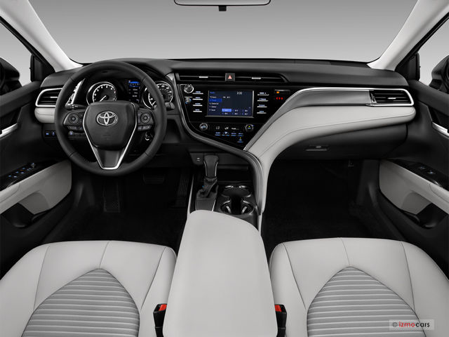
\includegraphics{images/dashboard.png}
This equivalent of a comfy coding environment is provided by the RStudio IDE (Integrated Developer Environment). We want you to install both R and RStudio, in that order.\\
Let's start with installing R.\\
R is free and available for download on the web. Go to the \href{https://r-project.org/}{r-project website} to get started.

This screen will look like this
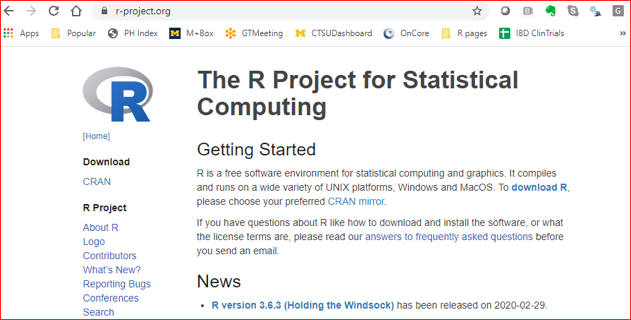
\includegraphics{images/r-project.png}\\
You can see from the blue link (download R) that you can download R, but you will be downloading it faster if you pick a local CRAN mirror.\\
You might be wondering what CRAN and CRAN Mirrors are. Nothing to do with cranberries, fortunately. CRAN is the Comprehensive R Archive Network. Each site (mirror) in the network contains an archive of all R versions and packages, and the sites are scattered over the globe. A CRAN Mirror maintains an up to date copy of all of the R versions and packages on CRAN. If you use the nearest CRAN mirror, you will generally get faster downloads.\\
At this point, you might be wondering what a package is\ldots{}\\
A package is a set of functions and/or data that you can download to upgrade and add features to R. It is a lot like a downloadable upgrade to a Tesla that lets you play the video game \emph{Witcher 3} on your console, but more useful.
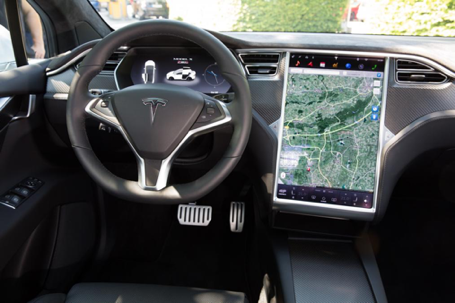
\includegraphics{images/dash-tesla.png}

Another useful analogy for packages is that they are like apps for a smartphone. When you buy your first smartphone, it only comes with the basic apps that allow it to work as a phone, but a notepad and a calculator.
If you want to do cool things with your smartphone, you download apps that allow your smartphone to have new capabilities. That is what packages do for your installation of R.
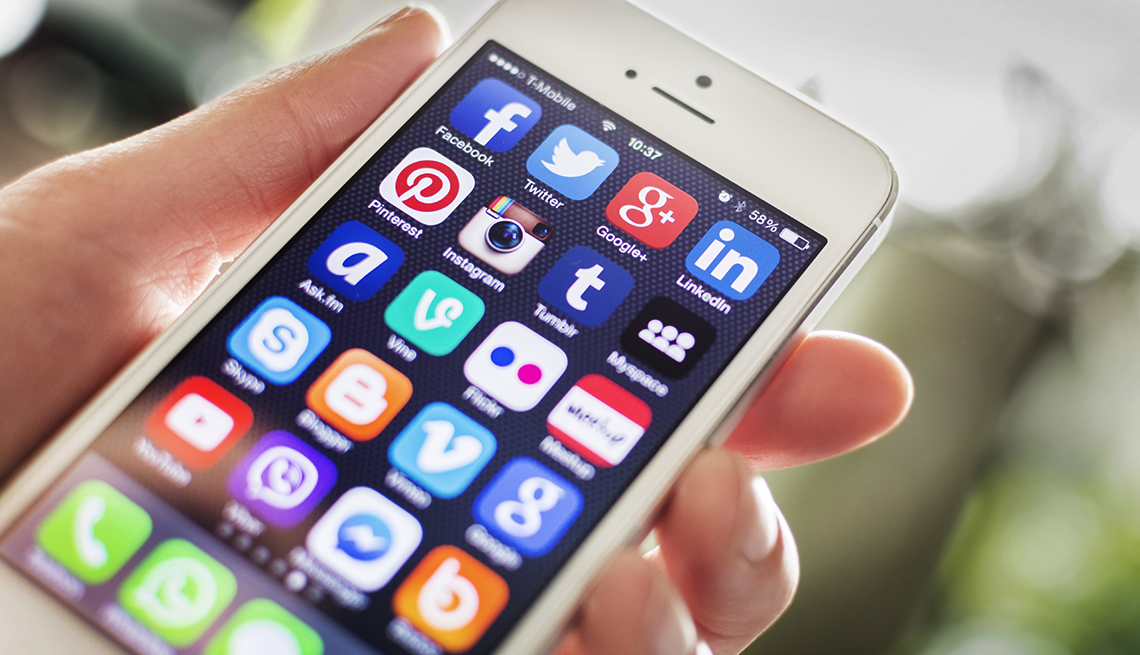
\includegraphics{images/smartphone.jpg}\\
Now let's get started. Click on the blue link that says ``download R''.\\
This will take you to a page to select your local CRAN Mirror , from which you will download R.
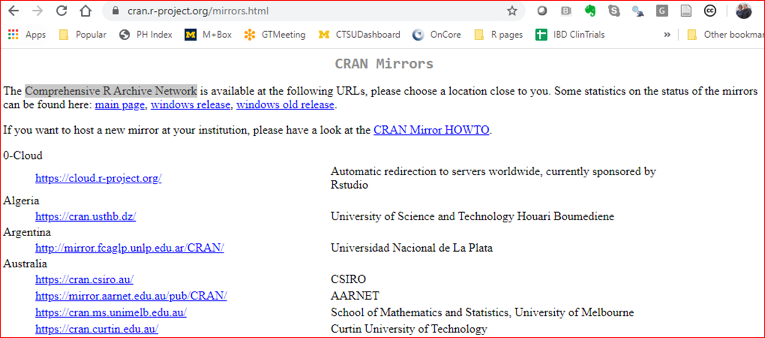
\includegraphics{images/cran-mirror.png}
Scroll down to your local country (yes, the USA is at the bottom), and a CRAN mirror near you.
This is an example from the state of Michigan, in the USA.
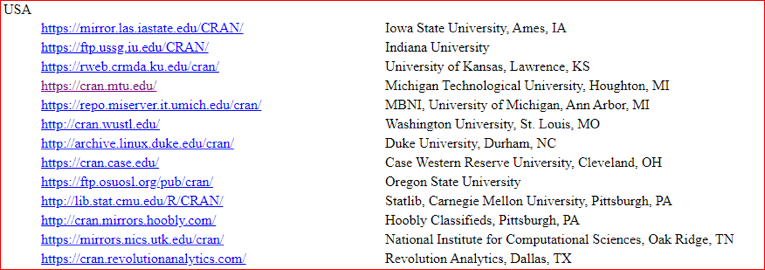
\includegraphics{images/usa-mirrors.png}
Once you click on a CRAN Mirror site to select the location, you will be taken to the actual Download site.
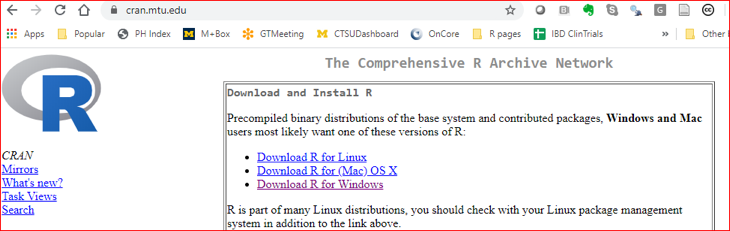
\includegraphics{images/installr.png}
Select the link for the operating system you want to use. We will walk through this with Windows first, then Mac. If you are using a Mac, skip forward to the Mac install directions. If you are computer-savvy enough to be using Linux, you can clearly figure it out on your own (it will look a lot like these).\\
Once you have clicked through, your next screen will look like this:\\
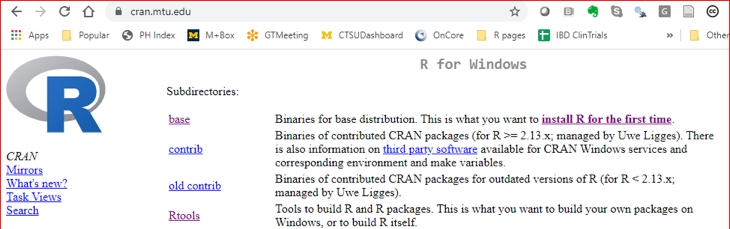
\includegraphics{images/installr2.png}
You want to download both base and Rtools (you might need Rtools later). The base link will take you to the latest version, which will look something like this.
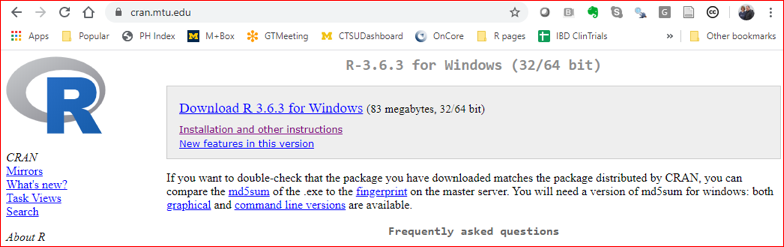
\includegraphics{images/installr3windows.png}
Click on this link, and you will be able to save a file named R-N.N.N-win.exe (Ns depending on version number) to your Downloads folder. Click on the Save button to save it.
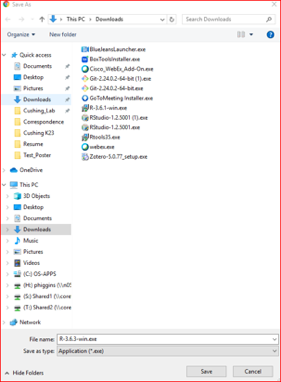
\includegraphics{images/installrsave.png}
Now, go to your Downloads folder in Windows, and double click on the R installation file (R-N.N.N-win.exe). Click Yes to allow this to install.
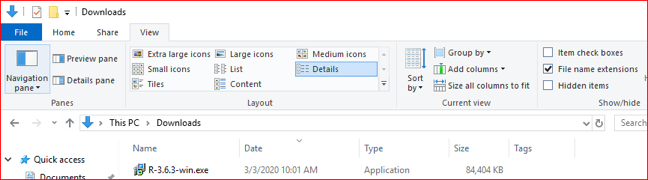
\includegraphics{images/installrexe.png}
Now select your language option.
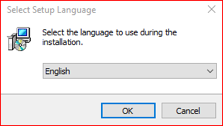
\includegraphics{images/installrEnglish.png}
You will be asked to accept the GNU license - do so. Click Yes to allow this to install. Then select where to install - generally use the default- a local (often C) drive - do not install on a shared network drive or in the cloud.
\includegraphics{images/installrdrive.png}
Then select the Components - generally use the defaults, but newer computers can skip the 32 bit version.
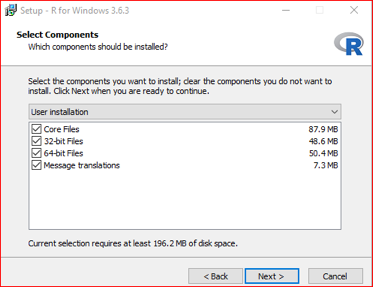
\includegraphics{images/installrComponents.png}
In the next dialog box, accept the default startup options.
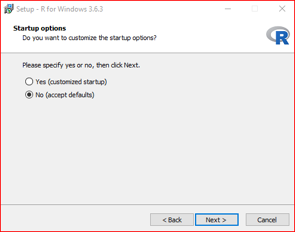
\includegraphics{images/installrdefaults.png}
You can choose the start menu folder. The default R folder is fine.
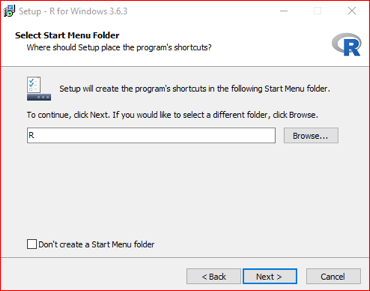
\includegraphics{images/installrstartmenu.png}
You probably won't need shortcuts, so leave these unchecked in the next dialog box.
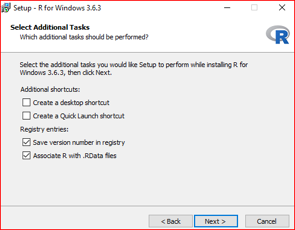
\includegraphics{images/installraddltasks.png}
Then the Setup Wizard will appear - click Finish, and the rest of the installation will occur.

\begin{figure}
\centering
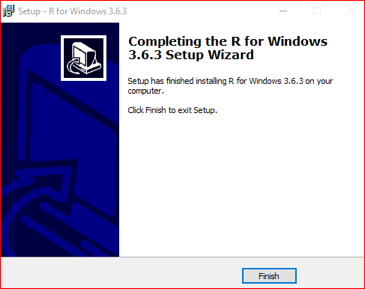
\includegraphics{images/installrwizard.png}
\caption{install\_wizard}
\end{figure}

\hypertarget{testing}{%
\subsection{Testing}\label{testing}}

Now you want to test whether your Windows installation was successful. Can you find R and make it work?
Hunt for your C folder, then for OS-APPS within that folder. Keep drilling down to the Program Files folder. Then the R folder, and the current version folder within that one (R-N.N.N). Within that folder will be the bin folder, and within that will be your R-N.N.N.exe file. Double click on this to run it. The example paths below can help guide you.
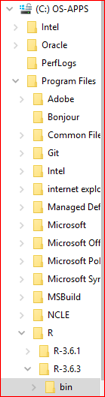
\includegraphics{images/installwin-path2.png}
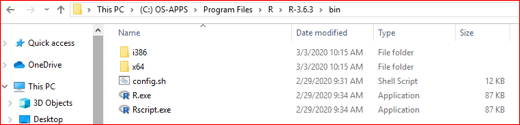
\includegraphics{images/installrpath.png}
Opening the exe file will produce a classic 2000-era terminal window, called Rterm, with 64 bit if that is what your computer uses. The version number should match what you downloaded. The messaging should end with a ``\textgreater{}'' prompt.
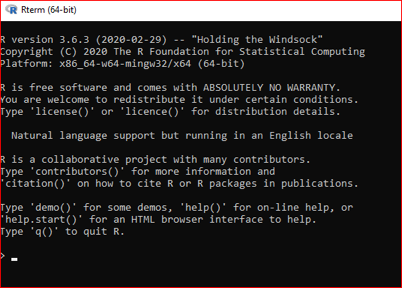
\includegraphics{images/windowsrterm.png}
At this prompt, type in:\\
paste(`Two to the seventh power is', 2\^{}7)
(don't leave out the comma) - then press the Enter key.

This should produce the following:

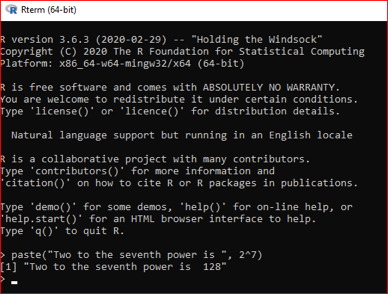
\includegraphics{images/windowstest.png}
Note that you have explained what is being done and computed the result.

\hypertarget{mac-install-of-r}{%
\subsection{Mac Install of R}\label{mac-install-of-r}}

The installation for Mac is very similar, but the windows look a bit different. At the Download Version page, you click on the Mac Download.
You will then click on the link for R-N.N.N.pkg, and allow downloads from CRAN.

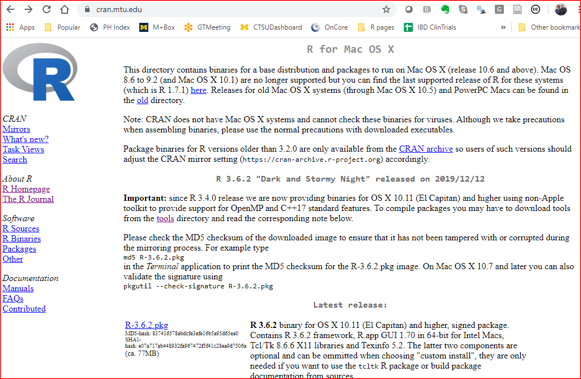
\includegraphics{images/installrpkgmac.png}
Then go to Finder, and navigate to the Downloads folder. Click on R-N.N.N.pkg
You will then click on the link for R-N.N.N.pkg, and allow downloads from CRAN.
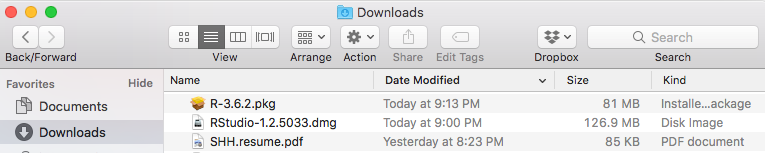
\includegraphics{images/installrdownloadsmac.png}

Click on Continue on 2 consecutive screens to download

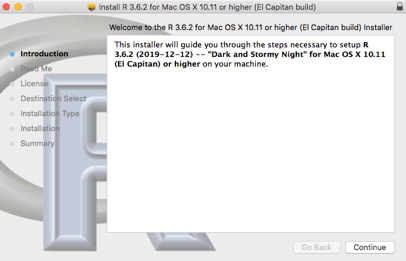
\includegraphics{images/installrCont1mac.png}

\begin{figure}
\centering
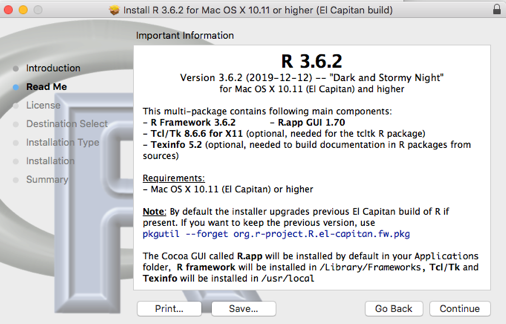
\includegraphics{images/installrCont2mac.png}
\caption{cont2\_mac}
\end{figure}

Then you need to agree with the License Agreement,
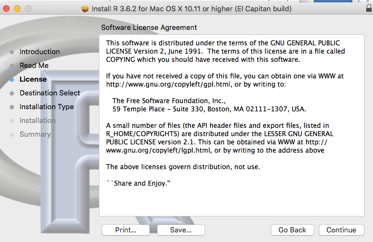
\includegraphics{images/installrmacLicense.png}
then Click on Install, and provide your Mac password for permission to install.
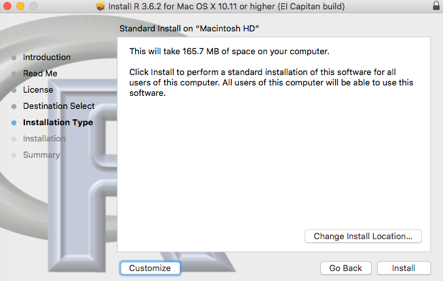
\includegraphics{images/installrmac-install.png}
When the installation is complete, click on the Close button. Accept the prompt to move the installer file to the trash.

\hypertarget{testing-r-on-the-mac}{%
\subsection{Testing R on the Mac}\label{testing-r-on-the-mac}}

Go to Finder, and then your Applications folder. Scroll down to the R file. Double click on this to run it.
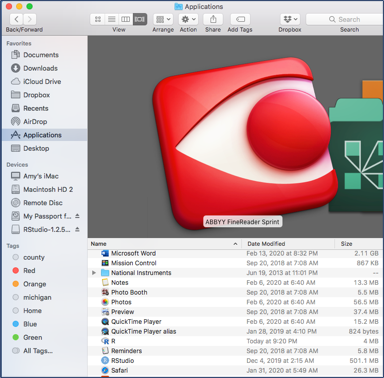
\includegraphics{images/findrmac.png}
You should get this 2000-era terminal window named R Console. The version number should match what you downloaded, and the messaging should end with a ``\textgreater{}'' prompt.
At this prompt, type in
paste(``Two to the seventh power is'', 2\^{}7)
(DON'T leave out the comma or the quotes)
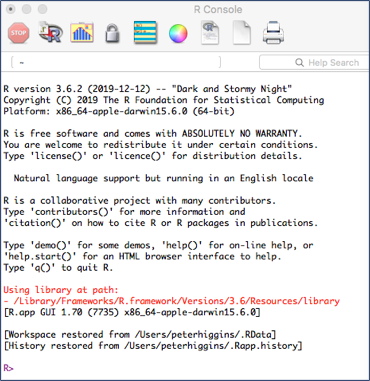
\includegraphics{images/rconsolemac.png}
This should result in
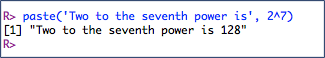
\includegraphics{images/mactestR.png}

\hypertarget{successful-testing}{%
\subsection{Successful testing!}\label{successful-testing}}

Awesome. You are now Ready to R!
\includegraphics{images/ready2R.png}

\hypertarget{installing-rstudio-on-your-computer}{%
\section{Installing RStudio on your Computer}\label{installing-rstudio-on-your-computer}}

Now that R is working, we will install RStudio. This is an IDE (Integrated Development Environment), with lots of bells and whistles to help you do reproducible medical research.
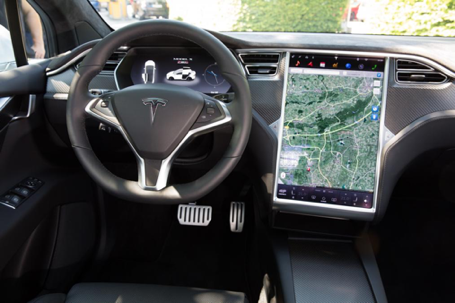
\includegraphics{images/teslax_dash.png}
This is a lot like adding a dashboard with polished walnut panels, a large video screen map, and heated car seats with Corinthian Leather. Not absolutely necessary, but nice to have.
The RStudio IDE wraps around the R engine to make your experience more comfortable and efficient.
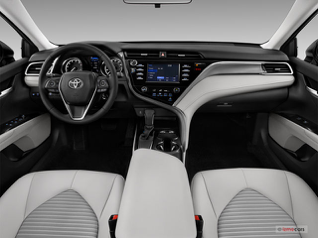
\includegraphics{images/camry_dash.png}
Fortunately, RStudio is a lot cheaper than any of these cars. In fact, it is free and open source. You can download it from the web at:
\href{https://rstudio.com/products/rstudio/}{rstudio}
Click on the RStudio Desktop icon to begin.

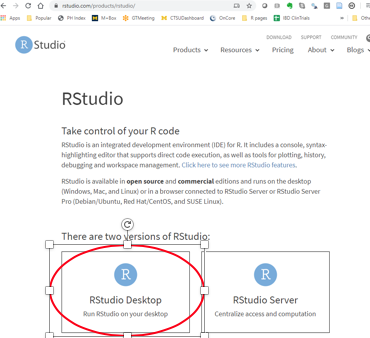
\includegraphics{images/rstudio_download.png}
This will take you to a new site, where you will select the Open Source Edition of RStudio Desktop

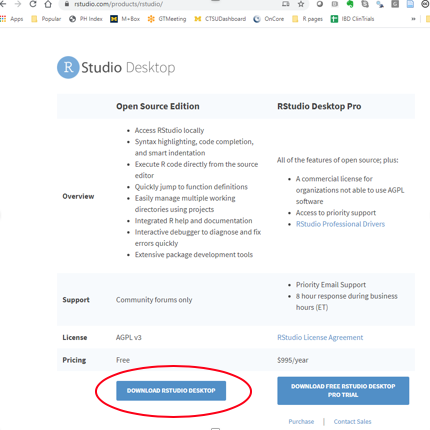
\includegraphics{images/rstudio_opensource.png}
This will take you to a new site, where you will select the Free Version of RStudio Desktop
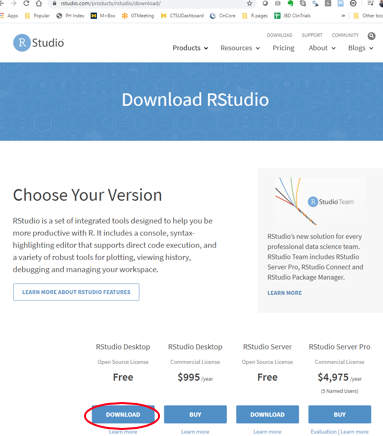
\includegraphics{images/rstudio_free.png}
Now select the right version for your Operating syxtem - Windows or Mac.
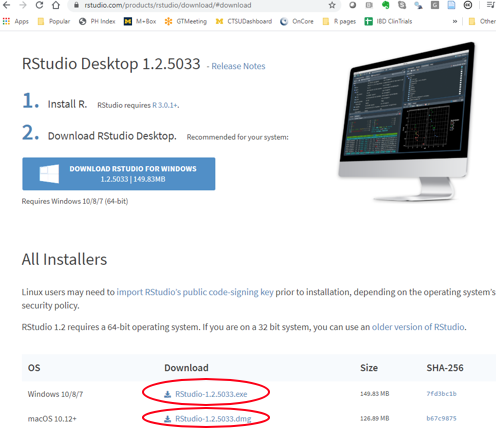
\includegraphics{images/rstudio_mac_win.png}

\hypertarget{windows-install}{%
\subsection{Windows Install}\label{windows-install}}

Now save the Rstudio.N.N.N.exe file (Ns will be digits representing the version number) to your downloads folder.
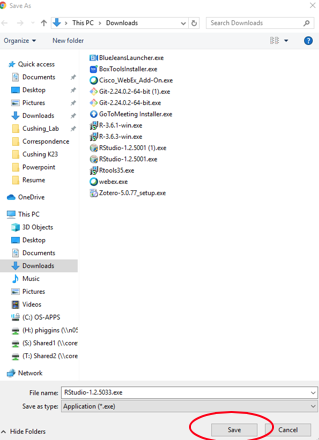
\includegraphics{images/rstudio_winsave.png}
Now go to your downloads folder, and double click on the Rstudio.N.N.N.exe file.
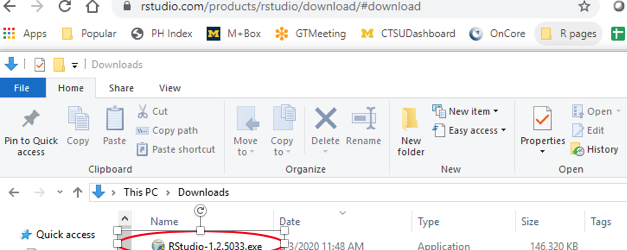
\includegraphics{images/rstudio_winlaunch.png}
Allow this app to make changes. Click Next to Continue, and Agree to the Install Location.
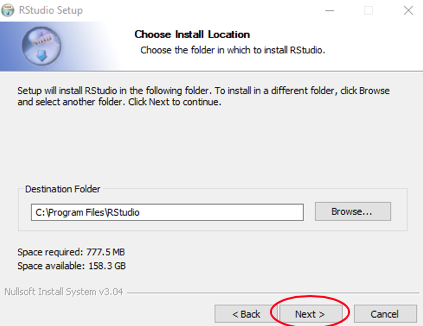
\includegraphics{images/rstudio_wininstall.png}
Click Install to put Rstudio in the default Start Menu Folder, and when done, click the Finish button.
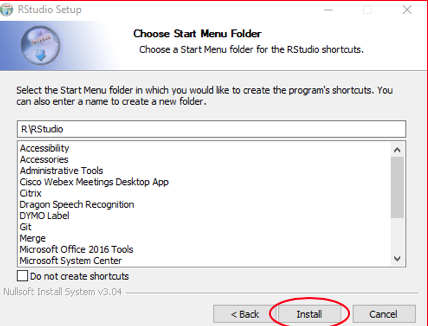
\includegraphics{images/rstudio_winstall_start.png}
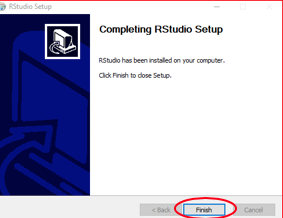
\includegraphics{images/winstall_finish.png}
Now select your preferred language option, accept the GNU license, Click Yes to allow this to install. Select where to install. This is generally on a local (often C:) drive, and usually \textbf{not} a shared network drive or in the cloud.

\hypertarget{testing-windows-rstudio}{%
\subsection{Testing Windows RStudio}\label{testing-windows-rstudio}}

Now you should be ready to test your Windows installation of Rstudio.
Open your Start menu Program list, and find Rstudio.
Pin it as a favorite now.
Click to Open Rstudio.
Within the Console window of Rstudio, an instance of R is started up. Check that the version number matches the version of R that you downloaded.
Now run a test at the prompt (``\textgreater{}'') in the Console window. Type in
\texttt{paste("Three\ to\ the\ 5th\ power\ is",\ 3\^{}5)}

\textbf{do not leave out the quotes or the comma}

Then press the enter key
and this should be your result:
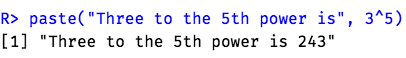
\includegraphics{images/test_result35.png}
A successful result means that you are ready to roll in Rstudio and R!
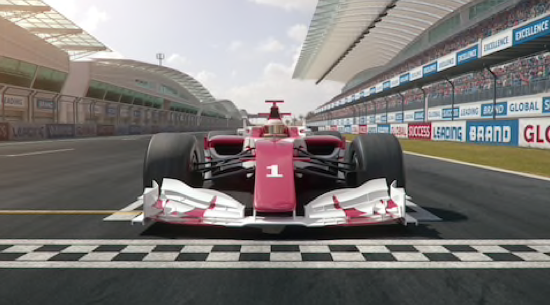
\includegraphics{images/ready_to_R.png}

\hypertarget{installing-rstudio-on-the-mac}{%
\subsection{Installing RStudio on the Mac}\label{installing-rstudio-on-the-mac}}

Start at this link: \href{https://rstudio.com/products/rstudio/download/}{Rstudio Download}
Select the Free RStudio Desktop Version
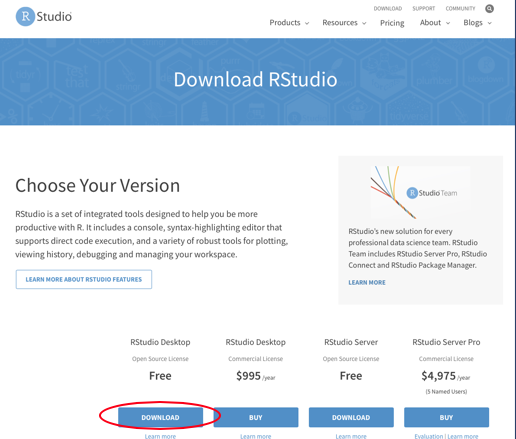
\includegraphics{images/rstudio_mac_download.png}
Then click on the big button to Download RStudio for Mac.
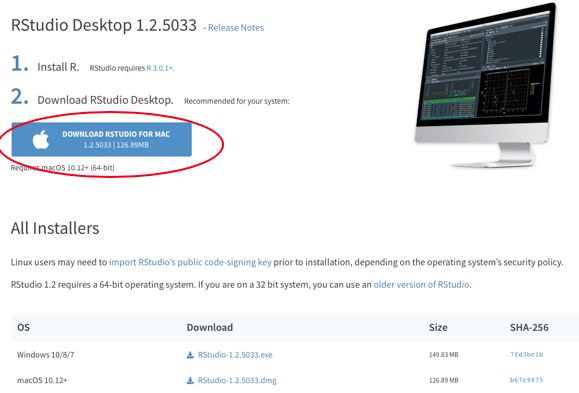
\includegraphics{images/rstudio_mac_download2.png}
After the Download is complete, go to Finder and the Downloads Folder. Double click on the Rstudio.N.N.N.dmg file in your Downloads folder.
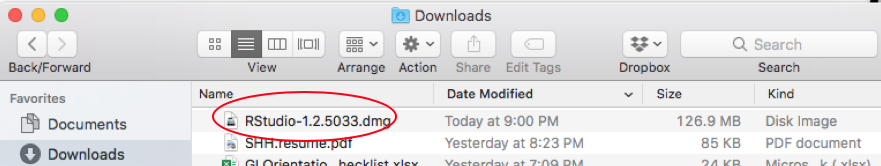
\includegraphics{images/rstudio_mac_dmg.png}
This will open a window that looks like this
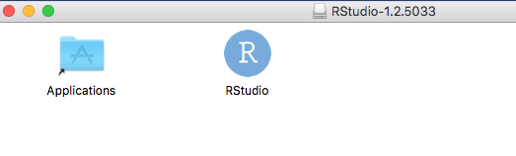
\includegraphics{images/rstudio_mac_apps.png}
Use your mouse to drag the RStudio icon into the Applications folder.
Now go back to Finder, then into the Applications folder.
Double click on the RStudio icon, and click OK to Open.
Pin your RStudio to the Dock.
Double Click to run RStudio.
RStudio will open an instance of R inside the Console pane of RStudio with the version number of R that you installed, and a ``\textgreater{}'' prompt.

\hypertarget{testing-the-mac-installation-of-rstudio}{%
\subsection{Testing the Mac Installation of RStudio}\label{testing-the-mac-installation-of-rstudio}}

Type in
\texttt{paste("Three\ to\ the\ 5th\ power\ is",\ 3\^{}5)}
\textbf{do not leave out the quotes or the comma}
Then press the enter key
and this should be your result.
\includegraphics{images/test_result35.png}
A successful result means that you are ready to roll in Rstudio and R!
\includegraphics{images/ready_to_R.png}

\hypertarget{installing-git-on-your-computer}{%
\section{Installing Git on your Computer}\label{installing-git-on-your-computer}}

\hypertarget{getting-acquainted-with-the-rstudio-ide}{%
\section{Getting Acquainted with the RStudio IDE}\label{getting-acquainted-with-the-rstudio-ide}}

\hypertarget{a-tasting-menu-of-r}{%
\chapter{A Tasting Menu of R}\label{a-tasting-menu-of-r}}

In this chapter, we will introduce you to a lot of neat things that you can do with R and RStudio, and you will publish a simple data analysis on the Internet
that you can share with friends and family.
\includegraphics{images/tasting.png}

\hypertarget{setting-the-table}{%
\section{Setting the Table}\label{setting-the-table}}

At the end of this chapter, you will publish a data analysis to \emph{RPubs}, a free website site where you can share your data analyses and visualizations. First you will need to set up an account on RPubs. Start by opening a new tab in your browser, and navigating to this \href{https://rpubs.com/users/new}{RPubs link}. It should look like the image below.
\includegraphics{images/rpubs1.png}\\
Enter your name, email, username and password, and click on the \emph{Register Now} button, and you will be set up to use RPubs.\\
This will bring you to this page. In the image below, we have set up an account for pdr.\\
\includegraphics{images/rpubs2.png}
Click on the \emph{Here's How You Get Started} link.
\includegraphics{images/rpubs3.png}\\
You are now all set up and ready to go. Now you have a place on the internet to share your R creations!

\hypertarget{goals-for-this-chapter-1}{%
\section{Goals for this Chapter}\label{goals-for-this-chapter-1}}

\begin{itemize}
\tightlist
\item
  Open a New Rmarkdown document
\item
  Read in Data from a file
\item
  Wrangle Your Data
\item
  Visualize Your Data
\item
  Publish your work to RPubs
\item
  Check out Interactive Plots
\item
  Check out Animated Graphics
\item
  Check out a Clinical Trial Dashboard
\item
  Check out a Shiny App
\end{itemize}

\hypertarget{packages-needed-for-this-chapter}{%
\section{Packages needed for this Chapter}\label{packages-needed-for-this-chapter}}

You will need to enter this line of code into your console, to make sure that the tidyverse package is installed on your computer.
\texttt{install.packages("tidyverse")}

In the setup chunk of your Rmarkdown document, you will need to access the tidyverse package with one line of code:
\texttt{library(tidyverse)}

\hypertarget{website-links-needed-for-this-chapter-1}{%
\section{Website links needed for this Chapter}\label{website-links-needed-for-this-chapter-1}}

In this chapter, you will need to access the RPubs website.\\
- \url{https://rpubs.com/}

\hypertarget{pathway-for-this-chapter-1}{%
\section{Pathway for this Chapter}\label{pathway-for-this-chapter-1}}

This Chapter is part of the \textbf{XXX} pathway.
Chapters in this pathway include

\hypertarget{open-a-new-rmarkdown-document}{%
\section{Open a New Rmarkdown document}\label{open-a-new-rmarkdown-document}}

Let's get started in R. Turn on your computer, and open the RStudio application. You should see the familiar panes for the Console, Environment, and Files.\\
You need to open up a new document to activate the Source pane. While in RStudio, click on File/New File/R Script.
It should look like this.\\
\includegraphics{images/rmd1.png}
Now you will see the window below. Rename the document from ``Untitled'' to ``Tasting'', and click the OK button.
\includegraphics{images/rmd2.png}

Now the file is open, and looks like the window below. Click on the save icon (like a floppy disk in the top left), and save this document as tasting.Rmd.
\includegraphics{images/rmd3.png}
You have created a new Rmarkdown document. An Rmarkdown document lets you mix data, code, and descriptive text. It is very helpful for presenting and explaining data and visualizations. An Rmarkdown document can be converted (Knit) to HTML for a web page, Microsoft Word, Powerpoint, PDF, and several other formats.

Code chunks are in a gray color, and both start and end with 3 backticks (```).

Text can be body text, or can be headers and titles. The number of hashtags before some header text defines what level the header is.\\
You can insert links, pictures, and YouTube videos into Rmarkdown documents if it is helpful to explain your point.
The first code chunk in each Rmarkdown document is named \texttt{setup}. The name comes after the left curly brace and the r (\texttt{\{r}) at the beginning of the setup chunk. The letter \texttt{r} tells RStudio that what is coming on the next line is R code (RStudio can also use SQL, C++, python, and several other languages). After the comma, you can define options for this code chunk. In this case, the option \texttt{include} is set to FALSE, so that when this Rmarkdown document is knitted, this code chunk will not appear.

\hypertarget{read-in-data-from-a-file}{%
\section{Read in Data from a file}\label{read-in-data-from-a-file}}

\hypertarget{wrangle-your-data}{%
\section{Wrangle Your Data}\label{wrangle-your-data}}

\hypertarget{visualize-your-data}{%
\section{Visualize Your Data}\label{visualize-your-data}}

\hypertarget{publish-your-work-to-rpubs}{%
\section{Publish your work to RPubs}\label{publish-your-work-to-rpubs}}

\hypertarget{the-dessert-cart}{%
\section{The Dessert Cart}\label{the-dessert-cart}}

Below are some examples of neat things you can do with medical data in R. These are more advanced approaches, but completely doable when you have more experience with R.

\hypertarget{interactive-plots}{%
\subsection{Interactive Plots}\label{interactive-plots}}

\hypertarget{animated-graphics}{%
\subsection{Animated Graphics}\label{animated-graphics}}

\hypertarget{a-clinical-trial-dashboard}{%
\subsection{A Clinical Trial Dashboard}\label{a-clinical-trial-dashboard}}

\hypertarget{a-shiny-app}{%
\subsection{A Shiny App}\label{a-shiny-app}}

\hypertarget{an-example-of-synergy-in-the-r-community}{%
\subsection{An Example of Synergy in the R Community}\label{an-example-of-synergy-in-the-r-community}}

One of the remarkable things about the open source R community is that people build all kinds of new R functions and packages that are useful to them, and then share them publicly with tools like \emph{Github} so that they can be useful to others. Often combining bits of several packages leads to \textbf{emergent properties} - completely new creations that can only occur because all of the parts (packages) are present. The collaborative nature of the R community, in this case on Twitter (follow the \#rstats hashtag), can lead to surprising collaborations and outcomes.\\
See the example below.\\

\hypertarget{updating-r-rstudio-and-your-packages}{%
\chapter{Updating R, RStudio, and Your Packages}\label{updating-r-rstudio-and-your-packages}}

This is an R Markdown document. Markdown is a simple formatting syntax for authoring HTML, PDF, and MS Word documents. For more details on using R Markdown see \url{http://rmarkdown.rstudio.com}.

\hypertarget{major-r-updates-where-are-my-packages}{%
\chapter{Major R Updates (Where Are My Packages?)}\label{major-r-updates-where-are-my-packages}}

This is an R Markdown document. Markdown is a simple formatting syntax for authoring HTML, PDF, and MS Word documents. For more details on using R Markdown see \url{http://rmarkdown.rstudio.com}.

\hypertarget{checking-validating-and-asserting-things-about-your-data}{%
\chapter{Checking, Validating, And Asserting things about your Data}\label{checking-validating-and-asserting-things-about-your-data}}

So you have imported your data!
Great!
Now to start the analysis!

Not so fast, cowboy!\\
First you need to validate your data.

\hypertarget{cleaning-names-with-janitor-package-to-snake_case}{%
\subsubsection{Cleaning -- names with janitor package to snake\_case}\label{cleaning-names-with-janitor-package-to-snake_case}}

\hypertarget{a-few-words-about-tidyverse-style}{%
\paragraph{A few words about tidyverse style}\label{a-few-words-about-tidyverse-style}}

\hypertarget{finding-missing-data-naniar-and-visdat-packages}{%
\subsubsection{Finding Missing data -- naniar and visdat packages}\label{finding-missing-data-naniar-and-visdat-packages}}

\hypertarget{validating-data-validate-package}{%
\subsubsection{Validating data -- validate package}\label{validating-data-validate-package}}

\hypertarget{asserting-properties-of-your-data-with-assertr}{%
\subsection{Asserting properties of your data with assertr}\label{asserting-properties-of-your-data-with-assertr}}

\hypertarget{evaluating-str-glimpse}{%
\subsubsection{Evaluating -- str, glimpse}\label{evaluating-str-glimpse}}

\hypertarget{exploring--skimr-package}{%
\subsubsection{Exploring- skimr package}\label{exploring--skimr-package}}

\hypertarget{histograms}{%
\subsubsection{Histograms}\label{histograms}}

\hypertarget{correlations-ggally-extension-of-ggplot2-and-corrr-package}{%
\subsubsection{Correlations -- ggally extension of ggplot2, and corrr package}\label{correlations-ggally-extension-of-ggplot2-and-corrr-package}}

\hypertarget{time-series-data-with-the-tidyverts-packages}{%
\chapter{Time Series data with the Tidyverts Packages}\label{time-series-data-with-the-tidyverts-packages}}

Fun text here.
All kinds of crazy examples.
Time series with data from influenza pandemic of 1918-19, perhaps.
This is a book for anyone in the medical field interested in analyzing the data available to them to better understand health, disease, or delivery of care. This could include nurses, dieticians, psychologists, and PhDs in related fields, as well as medical students, residents, fellows, or doctors in practice.\\
I expect that most learners will be using this book in their spare time at night and on weekends, as the medical school curriculum is already packed full, and there is no room to add skills in reproducible research to the standard curriculum. This book is designed for self-teaching, and many hints and solutions will be provided to avoid roadblocks and frustration.

\hypertarget{tsibble}{%
\section{Tsibble}\label{tsibble}}

Time series tibble

\href{https://tidyverts.org}{Tidyverts webpage}

\hypertarget{fable}{%
\section{Fable}\label{fable}}

Tidy forecasting

\hypertarget{feasts}{%
\section{Feasts}\label{feasts}}

Feature extraction and Statistics

\hypertarget{slider}{%
\section{Slider}\label{slider}}

Rolling anaylsis with window functions.\\
\href{https://davisvaughan.github.io/slider/}{Slider packagedown page}

\hypertarget{descriptive-data-tables}{%
\chapter{Descriptive Data Tables}\label{descriptive-data-tables}}

In this chapter, we will focus on making the descriptive table of the participants in your study, often colloquially know as ``Table One'', based on its usual placement in a medical manuscript.\\
Before we plunge in, I would like to make one point of warning. It is quite common in a multiple-arm randomized controlled trial to compare the distribution of particular baseline characteristics of the subjects between arms with a p value, usually in a column at the far right. This is silly, as this produces a whole column of p values, corresponding to the multiple comparisons performed. With 20 comparisons, by chance, you are likely to get one or more ``significant'' p values. These are not helpful or meaningful, and are considered bad statistical practice.\\
Let me quote the CONSORT guidelines on the publications of clinical trials.
\emph{``Unfortunately significance tests of baseline differences are still common; they were reported in half of 50 RCTs published in leading general journals in 1997. Such significance tests assess the probability that observed baseline differences could have occurred by chance; however, we already know that any differences are caused by chance. Tests of baseline differences are not necessarily wrong, just illogical. Such hypothesis\\
testing is superfluous and can mislead investigators and their readers. Rather, comparisons at baseline should be based on consideration of the prognostic strength of the variables measured and the size \textgreater of any chance imbalances that have occurred.''} \href{http://www.consort-statement.org/checklists/view/32-consort/510-\%3Ebaseline-data}{CONSORT STATEMENT}

Despite this, some journals and editors still ask for these p values. Please resist, and quote the CONSORT statement. If you must do this, please do it only under duress.

\hypertarget{making-table-one}{%
\section{Making Table One}\label{making-table-one}}

\hypertarget{the-tableby-function-in-the-arsenal-package}{%
\subsection{\texorpdfstring{The \emph{tableby} function in the \textbf{arsenal} package}{The tableby function in the arsenal package}}\label{the-tableby-function-in-the-arsenal-package}}

\hypertarget{the-gtsummary-package-with-flextable}{%
\subsection{The gtsummary package with flextable}\label{the-gtsummary-package-with-flextable}}

This is a newer approach which offers many of the same features as tableby. The gtsummary package is a companion to/built upon the gt package, (``gt'' for grammar of tables), which is supported by RStudio. The gtsummary package, like gt, is designed to produce nice html output with lots of nice formatting.
However, as a nice bonus, gtsummary includes a neat function \emph{as\_flextable}, which converts your resulting table into a flextable, which can be knit to a Microsoft Word Document or a Powerpoint presentation with Rmarkdown.
This means that you can make a table once, and be able to produce output in HTML for webpages, Microsoft Word for manuscripts, and MS Powerpoint for presentations from the same file without any conversion issues.
The only question is how and when you prefer to format your table. Both gt and flextable have great options for formatting your tables. You can do this in gt, then do \emph{as\_flextable}, or you can convert to a flextable first, then do your formatting. You can choose based on your comfort and familiarity with flextable vs.~gt. Both have excellent explanatory websites, with flextable \href{https://davidgohel.github.io/flextable/index.html}{here} and gtsummary \href{http://www.danieldsjoberg.com/gtsummary/index.html}{here}.

\hypertarget{making-an-adverse-events-table}{%
\section{Making An Adverse Events Table}\label{making-an-adverse-events-table}}

\hypertarget{making-a-results-table}{%
\section{Making A Results Table}\label{making-a-results-table}}

\hypertarget{comparing-two-measures-of-centrality}{%
\chapter{Comparing Two Measures of Centrality}\label{comparing-two-measures-of-centrality}}

A common question in medical research is whether one group had a better outcome than another group. These outcomes can be measured with dichotomous outcomes like death or hospitalization,
but continuous outcomes like systolic blood pressure, endoscopic score, or ejection fraction are more commonly available, and provide more statistical power, and usually require a smaller sample size.
There is a tendency in clinical research to focus on dichotomous outcomes, even to the point of converting continuous measures to dichotomous ones (aka ``dichotomania'', see Frank Harrell comments \href{http://biostat.mc.vanderbilt.edu/wiki/Main/CatContinuous}{here}), for fear of detecting and acting upon a small change in a continuous outcome that is not clinically meaningful.
While this can be a concern, especially in very large, over-powered studies, it can be addressed by aiming for a continuous difference that is at least as large as one that many clinicians agree (\emph{a priori}) is clinically important (the MCID, or Minimum Clinically Important Difference).
The most common comparison of two groups with a continuous outcome is to look at the means or medians, and determine whether the available evidence suggests that these are equal (the null hypothesis). This can be done for means with Student's t-test.
Let's start by looking at the cytomegalovirus data set. This includes data on 64 patients who received bone marrow stem cell transplant, and looks at their time to activation of CMV (cytomegalovirus). In the code chunk below, we group the data by donor cmv status (\texttt{donor.cmv}), and look at the mean time to CMV activation (\texttt{time.to.cmv} variable). Run the code (using the green arrow at the top right of the code chunk below) to see the difference in time to CMV activation in months between groups.

Try out some other grouping variables in the \texttt{group\_by} statement, in place of \texttt{donor.cmv}.
Consider variables like race, sex, and recipient.cmv. Edit the code and run it again with the green arrow at the top right.

\begin{verbatim}
## # A tibble: 2 x 2
##     sex mean_time2cmv
## * <dbl>         <dbl>
## 1     0          13.7
## 2     1          12.7
\end{verbatim}

That seems like a big difference for donor.cmv, between 13.7303333333333 months and 12.7441176470588 months. And it makes theoretical sense that having a CMV positive donor is more likely to be associated with early activation of CMV in the recipient. But is it a significant difference, one that would be very unlikely to happen by chance? That depends on things like the number of people in each group, and the standard deviation in each group. That is the kind of question you can answer with a t-test, or for particularly skewed data like hospital length of stay or medical charges, a Wilcoxon test.

\hypertarget{common-problem}{%
\section{Common Problem}\label{common-problem}}

\begin{itemize}
\tightlist
\item
  Comparing two groups

  \begin{itemize}
  \tightlist
  \item
    Mean or median vs.~expected
  \item
    Two arms of study - independent
  \item
    Pre and post / spouse and partner / left vs right arm -- paired groups
  \end{itemize}
\item
  Are the means significantly different?
\item
  Or the medians (if not normally distributed)?
\end{itemize}

\hypertarget{how-skewed-is-too-skewed}{%
\subsection{How Skewed is Too Skewed?}\label{how-skewed-is-too-skewed}}

\begin{itemize}
\tightlist
\item
  Formal test of normality = Shapiro-Wilk test
\item
  Use base data set called ToothGrowth
\end{itemize}

\begin{Shaded}
\begin{Highlighting}[]
\KeywordTok{library}\NormalTok{(tidyverse)}
\NormalTok{data <-}\StringTok{ }\NormalTok{cytomegalovirus}
\KeywordTok{head}\NormalTok{(data)}
\end{Highlighting}
\end{Shaded}

\begin{verbatim}
##   ID age sex race                    diagnosis
## 1  1  61   1    0       acute myeloid leukemia
## 2  2  62   1    1         non-Hodgkin lymphoma
## 3  3  63   0    1         non-Hodgkin lymphoma
## 4  4  33   0    1             Hodgkin lymphoma
## 5  5  54   0    1 acute lymphoblastic leukemia
## 6  6  55   1    1                myelofibrosis
##   diagnosis.type time.to.transplant prior.radiation
## 1              1               5.16               0
## 2              0              79.05               1
## 3              0              35.58               0
## 4              0              33.02               1
## 5              0              11.40               0
## 6              1               2.43               0
##   prior.chemo prior.transplant recipient.cmv donor.cmv
## 1           2                0             1         0
## 2           3                0             0         0
## 3           4                0             1         1
## 4           4                0             1         0
## 5           5                0             1         1
## 6           0                0             1         1
##   donor.sex TNC.dose CD34.dose CD3.dose CD8.dose TBI.dose
## 1         0    18.31      2.29     3.21     0.95      200
## 2         1     4.26      2.04       NA       NA      200
## 3         0     8.09      6.97     2.19     0.59      200
## 4         1    21.02      6.09     4.87     2.32      200
## 5         0    14.70      2.36     6.55     2.40      400
## 6         1     4.29      6.91     2.53     0.86      200
##   C1/C2 aKIRs cmv time.to.cmv agvhd time.to.agvhd cgvhd
## 1     0     1   1        3.91     1          3.55     0
## 2     1     5   0       65.12     0         65.12     0
## 3     0     3   0        3.75     0          3.75     0
## 4     0     2   0       48.49     1         28.55     1
## 5     0     6   0        4.37     1          2.79     0
## 6     0     2   1        4.53     1          3.88     0
##   time.to.cgvhd
## 1          6.28
## 2         65.12
## 3          3.75
## 4         10.45
## 5          4.37
## 6          6.87
\end{verbatim}

\hypertarget{visualize-the-distribution-of-data-variables-in-ggplot}{%
\subsection{Visualize the Distribution of data variables in ggplot}\label{visualize-the-distribution-of-data-variables-in-ggplot}}

\begin{itemize}
\tightlist
\item
  Use geom\_histogram or geom\_density (pick one or the other)
\item
  look at the distribution of CD3.dose or time.to.cmv
\item
  Bonus points: facet by sex or race or donor.cmv
\item
  Your turn to try it
\end{itemize}

\includegraphics{io30-ttest_files/figure-latex/density-1.pdf}

\begin{Shaded}
\begin{Highlighting}[]
\NormalTok{data }\OperatorTok\StringTok{ }
\KeywordTok{ggplot}\NormalTok{(}\DataTypeTok{mapping =} \KeywordTok{aes}\NormalTok{(time.to.cmv)) }\OperatorTok{+}
\StringTok{  }\KeywordTok{geom_histogram}\NormalTok{() }\OperatorTok{+}
\StringTok{  }\KeywordTok{facet_wrap}\NormalTok{(}\OperatorTok{~}\NormalTok{race)}
\end{Highlighting}
\end{Shaded}

\includegraphics{io30-ttest_files/figure-latex/histogram-1.pdf}

\hypertarget{visualize-the-distribution-of-datalen-in-ggplot}{%
\subsection{Visualize the Distribution of data\$len in ggplot}\label{visualize-the-distribution-of-datalen-in-ggplot}}

\begin{itemize}
\tightlist
\item
  The OJ group is left skewed
\item
  May be problematic for using means
\item
  formally test with Shapiro-Wilk
\end{itemize}

\begin{Shaded}
\begin{Highlighting}[]
\NormalTok{data}\OperatorTok{$}\NormalTok{time.to.cmv }\OperatorTok\StringTok{ }
\KeywordTok{shapiro.test}\NormalTok{()}
\end{Highlighting}
\end{Shaded}

\begin{verbatim}
## 
##  Shapiro-Wilk normality test
## 
## data:  .
## W = 0.68261, p-value = 0.0000000001762
\end{verbatim}

\hypertarget{results-of-shapiro-wilk}{%
\subsection{Results of Shapiro-Wilk}\label{results-of-shapiro-wilk}}

\begin{itemize}
\tightlist
\item
  p-value = 0.1091
\item
  p not \textless{} 0.05
\item
  Acceptably close to normal
\item
  OK to compare means rather than medians
\item
  can use t test rather than wilcoxon test

  \begin{itemize}
  \tightlist
  \item
    if p is \textless{} 0.05, use wilcoxon test
  \item
    also known as Mann-Whitney test
  \item
    a rank-based (non-parametric) test
  \end{itemize}
\end{itemize}

\hypertarget{try-it-yourself}{%
\subsection{Try it yourself}\label{try-it-yourself}}

\begin{itemize}
\tightlist
\item
  use df \textless- msleep
\end{itemize}

\begin{Shaded}
\begin{Highlighting}[]
\NormalTok{df <-}\StringTok{ }\NormalTok{msleep }
\KeywordTok{head}\NormalTok{(df}\OperatorTok{$}\NormalTok{sleep_total)}
\end{Highlighting}
\end{Shaded}

\begin{verbatim}
## [1] 12.1 17.0 14.4 14.9  4.0 14.4
\end{verbatim}

\begin{itemize}
\tightlist
\item
  test the normality of total sleep hours in mammals
\end{itemize}

\hypertarget{mammal-sleep-hours}{%
\subsection{Mammal sleep hours}\label{mammal-sleep-hours}}

\begin{Shaded}
\begin{Highlighting}[]
\KeywordTok{shapiro.test}\NormalTok{(df}\OperatorTok{$}\NormalTok{sleep_total)}
\end{Highlighting}
\end{Shaded}

\begin{verbatim}
## 
##  Shapiro-Wilk normality test
## 
## data:  df$sleep_total
## W = 0.97973, p-value = 0.2143
\end{verbatim}

\begin{itemize}
\tightlist
\item
  meets criteria - acceptable to consider normally distributed
\item
  now consider - is the mean roughly 8 hours of sleep per day?
\end{itemize}

\hypertarget{one-sample-t-test}{%
\section{One Sample T test}\label{one-sample-t-test}}

\begin{itemize}
\tightlist
\item
  univariate test

  \begin{itemize}
  \tightlist
  \item
    Ho: mean is 8 hours
  \item
    Ha: mean is not 8 hours
  \end{itemize}
\item
  can use t test because shapiro.test is NS
\end{itemize}

\hypertarget{how-to-do-one-sample-t-test}{%
\subsection{How to do One Sample T test}\label{how-to-do-one-sample-t-test}}

\begin{Shaded}
\begin{Highlighting}[]
\KeywordTok{t.test}\NormalTok{(df}\OperatorTok{$}\NormalTok{sleep_total, }\DataTypeTok{alternative =} \StringTok{"two.sided"}\NormalTok{,}
       \DataTypeTok{mu =} \DecValTok{8}\NormalTok{)}
\end{Highlighting}
\end{Shaded}

\begin{itemize}
\tightlist
\item
  Try it out, see if you can interpret results
\end{itemize}

\hypertarget{interpreting-the-one-sample-t-test}{%
\subsection{Interpreting the One Sample T test}\label{interpreting-the-one-sample-t-test}}

\begin{verbatim}
## 
##  One Sample t-test
## 
## data:  df$sleep_total
## t = 4.9822, df = 82, p-value = 0.000003437
## alternative hypothesis: true mean is not equal to 8
## 95 percent confidence interval:
##   9.461972 11.405497
## sample estimates:
## mean of x 
##  10.43373
\end{verbatim}

\begin{itemize}
\tightlist
\item
  p is highly significant

  \begin{itemize}
  \tightlist
  \item
    can reject the null, accept alternative
  \item
    sample mean 10.43, CI 9.46-11.41
  \end{itemize}
\end{itemize}

\hypertarget{what-are-the-arguments-of-the-t.test-function}{%
\subsection{What are the arguments of the t.test function?}\label{what-are-the-arguments-of-the-t.test-function}}

\begin{itemize}
\tightlist
\item
  x = vector of continuous numerical data
\item
  y= NULL - optional 2nd vector of continuous numerical data
\item
  alternative = c(``two.sided'', ``less'', ``greater''),
\item
  mu = 0
\item
  paired = FALSE
\item
  var.equal = FALSE
\item
  conf.level = 0.95
\item
  \href{https://www.rdocumentation.org/packages/stats/versions/3.5.1/topics/t.test}{documentation}
\end{itemize}

\hypertarget{fine-but-what-about-2-groups}{%
\section{Fine, but what about 2 groups?}\label{fine-but-what-about-2-groups}}

\begin{itemize}
\tightlist
\item
  consider df\$vore
\end{itemize}

\begin{Shaded}
\begin{Highlighting}[]
\KeywordTok{table}\NormalTok{(df}\OperatorTok{$}\NormalTok{vore)}
\end{Highlighting}
\end{Shaded}

\begin{verbatim}
## 
##   carni   herbi insecti    omni 
##      19      32       5      20
\end{verbatim}

\begin{itemize}
\tightlist
\item
  hypothesis - herbivores need more time to get food, sleep less than carnivores
\item
  how to test this?

  \begin{itemize}
  \tightlist
  \item
    normal, so can use t test for 2 groups
  \end{itemize}
\end{itemize}

\hypertarget{setting-up-2-group-t-test}{%
\subsection{Setting up 2 group t test}\label{setting-up-2-group-t-test}}

\begin{itemize}
\tightlist
\item
  formula interface: outcome \textasciitilde{} groupvar
\end{itemize}

\begin{Shaded}
\begin{Highlighting}[]
\NormalTok{df }\OperatorTok\StringTok{ }
\StringTok{  }\KeywordTok{filter}\NormalTok{(vore }\OperatorTok\StringTok{ }\KeywordTok{c}\NormalTok{(}\StringTok{"herbi"}\NormalTok{, }\StringTok{"carni"}\NormalTok{)) }\OperatorTok\StringTok{ }
\StringTok{  }\KeywordTok{t.test}\NormalTok{(}\DataTypeTok{formula =}\NormalTok{ sleep_total }\OperatorTok{~}\StringTok{ }\NormalTok{vore, }\DataTypeTok{data =}\NormalTok{ .)}
\end{Highlighting}
\end{Shaded}

\begin{itemize}
\tightlist
\item
  Try it yourself
\item
  What do the results mean?
\end{itemize}

\hypertarget{results-of-the-2-group-t-test}{%
\subsection{Results of the 2 group t test}\label{results-of-the-2-group-t-test}}

\begin{verbatim}
## 
##  Welch Two Sample t-test
## 
## data:  sleep_total by vore
## t = 0.63232, df = 39.31, p-value = 0.5308
## alternative hypothesis: true difference in means is not equal to 0
## 95 percent confidence interval:
##  -1.911365  3.650509
## sample estimates:
## mean in group carni mean in group herbi 
##           10.378947            9.509375
\end{verbatim}

\hypertarget{interpreting-the-2-group-t-test}{%
\subsection{Interpreting the 2 group t test}\label{interpreting-the-2-group-t-test}}

\begin{itemize}
\tightlist
\item
  Welch t-test (not Student)

  \begin{itemize}
  \tightlist
  \item
    Welch does NOT assume equal variances in each group
  \end{itemize}
\item
  p value NS
\item
  accept null hypothesis

  \begin{itemize}
  \tightlist
  \item
    Ho: means of groups roughly equal
  \item
    Ha: means are different
  \item
    95\% CI crosses 0
  \end{itemize}
\item
  Carnivores sleep a little more, but not a lot
\end{itemize}

\hypertarget{group-t-test-with-wide-data}{%
\subsection{2 group t test with wide data}\label{group-t-test-with-wide-data}}

\begin{itemize}
\tightlist
\item
  You want to compare column A with column B (data are not tidy)
\item
  Do mammals spend more time awake than asleep?
\end{itemize}

\begin{Shaded}
\begin{Highlighting}[]
\KeywordTok{t.test}\NormalTok{(}\DataTypeTok{x =}\NormalTok{ df}\OperatorTok{$}\NormalTok{sleep_total, }\DataTypeTok{y =}\NormalTok{ df}\OperatorTok{$}\NormalTok{awake, }\DataTypeTok{data =}\NormalTok{ msleep)}
\end{Highlighting}
\end{Shaded}

\hypertarget{results-of-2-group-t-test-with-wide-data}{%
\subsection{Results of 2 group t test with wide data}\label{results-of-2-group-t-test-with-wide-data}}

\begin{Shaded}
\begin{Highlighting}[]
\KeywordTok{t.test}\NormalTok{(}\DataTypeTok{x =}\NormalTok{ df}\OperatorTok{$}\NormalTok{sleep_total, }\DataTypeTok{y =}\NormalTok{ df}\OperatorTok{$}\NormalTok{awake, }\DataTypeTok{data =}\NormalTok{ msleep)}
\end{Highlighting}
\end{Shaded}

\begin{verbatim}
## 
##  Welch Two Sample t-test
## 
## data:  df$sleep_total and df$awake
## t = -4.5353, df = 164, p-value = 0.00001106
## alternative hypothesis: true difference in means is not equal to 0
## 95 percent confidence interval:
##  -4.498066 -1.769404
## sample estimates:
## mean of x mean of y 
##  10.43373  13.56747
\end{verbatim}

\hypertarget{assumptions-of-students-t-test}{%
\section{3 Assumptions of Student's t test}\label{assumptions-of-students-t-test}}

\begin{enumerate}
\def\labelenumi{\arabic{enumi}.}
\tightlist
\item
  Sample is normally distributed (test with Shapiro)
\item
  Variances are homogeneous (homoskedasticity) (test with Levene)
\item
  Observations are independent
\end{enumerate}

\begin{itemize}
\tightlist
\item
  not paired like left vs.~right colon
\item
  not paired like spouse and partner
\item
  not paired like measurements pre and post Rx
\end{itemize}

\hypertarget{testing-assumptions-of-students-t-test}{%
\subsection{Testing Assumptions of Student's t test}\label{testing-assumptions-of-students-t-test}}

\begin{itemize}
\tightlist
\item
  Normality - test with Shapiro

  \begin{itemize}
  \tightlist
  \item
    If not normal, Wilcoxon \textgreater{} t test
  \end{itemize}
\item
  Equal Variances - test with Levene

  \begin{itemize}
  \tightlist
  \item
    If not equal, Welch t \textgreater{} Student's t
  \end{itemize}
\item
  Observations are independent

  \begin{itemize}
  \tightlist
  \item
    Think about data collection
  \item
    are some observations correlated with some others?
  \item
    If correlated, use paired t test
  \end{itemize}
\end{itemize}

\hypertarget{getting-results-out-of-t.test}{%
\section{Getting results out of t.test}\label{getting-results-out-of-t.test}}

\begin{itemize}
\tightlist
\item
  Use the tidy function from the broom package
\item
  Do carnivores have bigger brains than insectivores?
\end{itemize}

\begin{Shaded}
\begin{Highlighting}[]
\NormalTok{df }\OperatorTok\StringTok{ }
\StringTok{  }\KeywordTok{filter}\NormalTok{(vore }\OperatorTok\StringTok{ }\KeywordTok{c}\NormalTok{(}\StringTok{"carni"}\NormalTok{, }\StringTok{"insecti"}\NormalTok{)) }\OperatorTok\StringTok{ }
\KeywordTok{t.test}\NormalTok{(}\DataTypeTok{formula =}\NormalTok{ brainwt }\OperatorTok{~}\StringTok{ }\NormalTok{vore, }\DataTypeTok{data =}\NormalTok{ .) }\OperatorTok\StringTok{ }
\StringTok{  }\KeywordTok{tidy}\NormalTok{() ->}
\NormalTok{result}
\NormalTok{result}
\end{Highlighting}
\end{Shaded}

\hypertarget{getting-results-out-of-t.test-1}{%
\subsection{Getting results out of t.test}\label{getting-results-out-of-t.test-1}}

\begin{verbatim}
## # A tibble: 1 x 9
##   estimate1 estimate2 statistic p.value parameter conf.low
##       <dbl>     <dbl>     <dbl>   <dbl>     <dbl>    <dbl>
## 1    0.0793    0.0216      1.20   0.253        12  -0.0471
## # ... with 3 more variables: conf.high <dbl>, method <chr>,
## #   alternative <chr>
\end{verbatim}

\hypertarget{reporting-the-results-from-t.test-using-inline-code}{%
\section{Reporting the results from t.test using inline code}\label{reporting-the-results-from-t.test-using-inline-code}}

\begin{itemize}
\tightlist
\item
  use backticks before and after, start with r

  \begin{itemize}
  \tightlist
  \item
    i.e.~My result is {[}backtick{]}r code here{[}backtick{]}.
  \end{itemize}
\item
  The mean brain weight for carnivores was 0.0792556
\item
  The mean brain weight for herbivores was 0.02155

  \begin{itemize}
  \tightlist
  \item
    The difference was
  \end{itemize}
\item
  The t statistic for this Two Sample t-test was 1.1995501
\item
  The p value was 0.2534631

  \begin{itemize}
  \tightlist
  \item
    The confidence interval was from -0.05 to 0.16
  \end{itemize}
\end{itemize}

\hypertarget{for-next-time}{%
\subsection{For Next Time}\label{for-next-time}}

\begin{itemize}
\tightlist
\item
  Skewness and Kurtosis
\item
  Review Normality

  \begin{itemize}
  \tightlist
  \item
    When to use Wilcoxon
  \end{itemize}
\item
  Levene test for equal variances

  \begin{itemize}
  \tightlist
  \item
    When to use Welch t vs.~Student's t
  \end{itemize}
\item
  Paired t and Wilcoxon tests
\end{itemize}

\hypertarget{title-holder}{%
\chapter*{Title holder}\label{title-holder}}
\addcontentsline{toc}{chapter}{Title holder}

  \bibliography{book.bib,packages.bib}

\end{document}
